% Paper template for TAR 2016
% (C) 2014 Jan Šnajder, Goran Glavaš, Domagoj Alagić, Mladen Karan
% TakeLab, FER

\documentclass[10pt, a4paper]{article}

\usepackage{tar2016}

\usepackage[utf8]{inputenc}
\usepackage[pdftex]{graphicx}
\usepackage{booktabs}
\usepackage{amsmath}
\usepackage{amssymb}

\title{Humor Detection and Ranking}

\name{Bartol Freškura, Filip Gulan, Damir Kopljar}

\address{
University of Zagreb, Faculty of Electrical Engineering and Computing\\
Unska 3, 10000 Zagreb, Croatia\\
\texttt{\{bartol.freskura, filip.gulan, damir.kopljar\}@fer.hr}\\
}

\abstract{ 
In this paper, we consider the task of comparative humor ranking in two manner:
detecting which tweet of two is more humorous and ranking the given tweets by how
humorous they are in three classes. We opted for different approaches based on
recent deep neural models in order to eschew manual feature engineering. In
evaluation section we experimented with the bi-directional LSTMs and CNNs, in
combination and separately. For constructing feature vectors we used
pre-trained Twitter \emph{GloVe} word embeddings along with trained character
embedding. The system was trained, tuned, and evaluated on the SemEval-2017 Task 6 dataset
for which it yields outstanding results.
}

\begin{document}

\maketitleabstract

\section{Introduction}

Understanding humor expressed in the text is a challenging natural language problem which has not yet been addressed extensively in the current AI research. Humor is often subjective and relies on the vast knowledge base, which is sometimes hard to reason, even for humans. It is also important to say that what is humorous today might not be humorous tomorrow due to the fact that humor can be trend dependent.

In this paper, we describe a system for humor detection and
ranking. Our system is designed to solve two tasks. For the first task, the
system is given two tweets and it should predict the funnier tweet.
For the second task, the system is given a set of tweets and it should rank them
in three categories (2 for the most humorous tweet, 1 for top ten humorous
tweets, and 0 otherwise). To learn and test our model we used a novel dataset that was
given in SemEval-2017 Task 6 \citep{potash2016hashtagwars}. The dataset consists of
the tweets that viewers sent as a part of the Comedy Central show @midnight. For every
episode, topic was defined and viewers were asked to send humorous
tweets on the given topic.

\section{Related Work}

In the last few years there were a lot of approaches in humor detection \citep{mihalcea2005,reyes2013,zhang2014,barbieri2014,yang2015}.
Some of those works \citep{reyes2013,zhang2014,barbieri2014} have also acquired
humor dataset from Twitter. Most of the related works separate the apprehension 
of humor into two groups: humor and non-humor, basically a binary classification.
This representation ignores the continuous nature of humor, while also not accounting
for the subjectivity in perceiving humor \citep{potash2016hashtagwars}.

SemEval-2017 Task 6 has finished in February, 2017 and most of the top-ranked participants \citep{humorhawk2017,takelab2017,datastories2017} published their work describing used techniques and models.

Donahue et al. with \emph{HumorHawk} team have won the contest on Task A (no data available for Task B). Their system utilizes recurrent deep learning methods with dense embeddings. They used \emph{GloVe} embeddings in combination with a novel phonetic representation which is used as input to LSTM. After LSTM, they have stacked character-based CNN model, and an XGBoost \citep{XGBoost2016} component in an ensemble model which achieves 0.675 accuracy on the evaluation data for the Task A.

Kukova\v{c}ec et al. with \emph{TakeLab} team have participated on both tasks, A and B, and have won the second place on both of them. Unlike the other two teams \citep{humorhawk2017,datastories2017}, which used deep-learning models with automatic feature extraction, they used a manually handcrafted rich set of features:  cultural reference features, binary and count-based features, readability-based features, humor-specific features and sentiment-based features. As a classifier they used gradient boosting model which achieves 0.641 accuracy on the evaluation data for the Task A, and distance of 0.908 on Task B evaluation data (lower is better, starting from 1).

Baziotis et al. with \emph{DataStories} team have won the third place on Task A (no data available for Task B). For their system they have used Siamese architecture \citep{siamese1993} with bidirectional LSTMs, augmented with an attention mechanism. Their model leverage word embeddings trained on big collection of unlabeled Twitter messages. Their system achieves 0.632 accuracy on the evaluation data for the Task A.

\section{Architecture}

In this section, we describe the architecture of our system. Our most complex
architecture consists of the bi-directional
\emph{Long Short Term Memory} \citep{lstm1997} layer, further referred as Bi-LSTM,
convolutional layer \citep{cnn1998}, further referred as CNN, and a fully connected
layer with a softmax layer at the end for predicting class probabilities.

The whole pipeline was built using the open source frameworks
\emph{TensorFlow} \footnote{\texttt{https://www.tensorflow.org/}} \citep{tensorflow2015}
and
\emph{scikit-learn} \footnote{\texttt{http://scikit-learn.org/stable/index.html}} \citep{scikit-learn}.

\subsection{Recurrent Neural Networks}

The main idea behind RNNs lies in retaining information from "history". In the 
context of NLP, history refers to observing the context of the sentence up to the
currently processed word. Despite the promising results in short sentences, RNN
losses its performance dramatically with the increasing sentence length due to 
the gradient vanishing \citep{bengio1994learning} and exploding problems 
\citep{pascanu2013difficulty}. LSTMs were designed with the purpose of correcting 
the RNNs shortcomings. Although LSTM can successfully capture the past context,
it is sometimes good to have an insight at the future sentence context. Bi-LSTMs 
model implements this by adding an extra LSTM layer which has a reversed information flow
meaning that the information is propagated from the end of the sentence towards
the beginning. Output of a Bi-LSTM is a concatenated vector of the two opposite LSTM layers.

\subsection{Convolutional Neural Networks}
CNN networks are famous for their appliance in the \emph{Computer Vision}
domain but have also demonstrated an ability to extract morphological information
from word characters, encoding them into neural representations. We first create
a hash map of all characters that appear in the dataset where values are arbitrarily
assigned integer values. All sentence characters are then represented using their
mapped integer values but the padding is also applied on the word level as shown
in Figure \ref{fig:cnn_embed}. Encoded sentence represents an input which is fed
into a trainable character embedding layer of $C_e \times V$ dimensions, where
$C_e$ is the character embedding size, and $V$ is the number of unique
characters in the corpus.

\begin{figure}
  \caption{Word embeddings and the CNN architecture}
  \label{fig:cnn_embed}
  \centering
    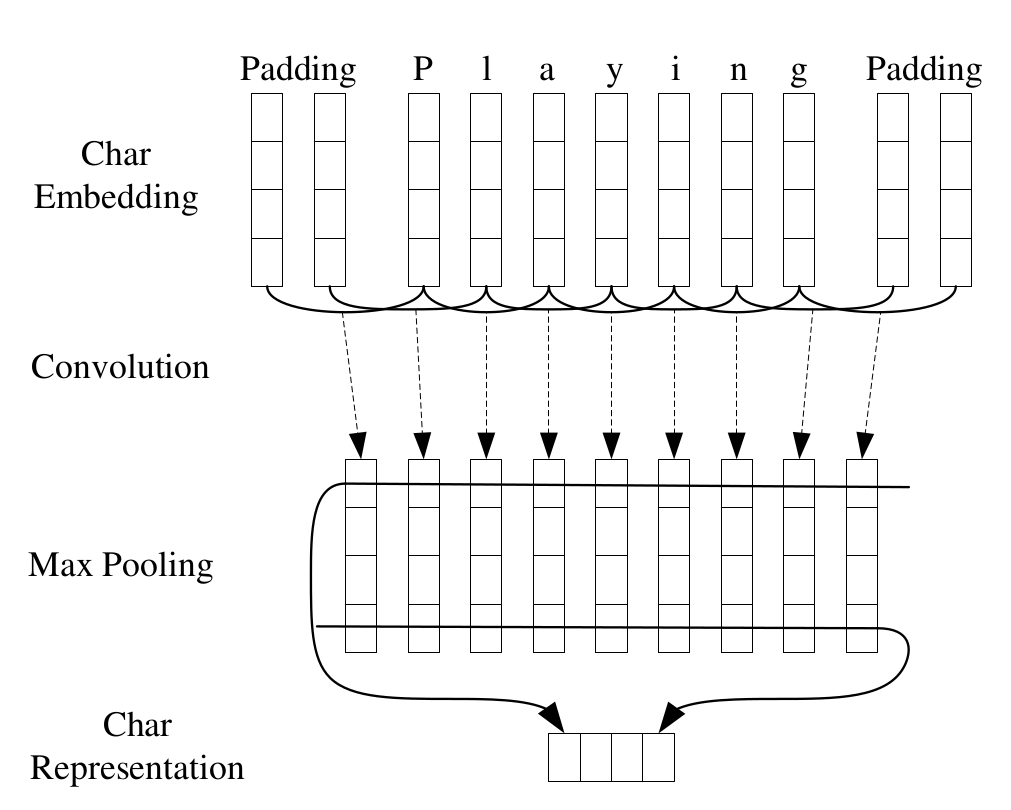
\includegraphics[width=0.4\textwidth]{imgs/cnn_embed.png}
\end{figure}

\subsection{Used models}

\subsubsection{CNN network}
Previous work \citep{potash2016hashtagwars} has demonstrated that CNN are top performers
when it comes to capturing humor. Our first model consists of the character
embedding layer followed by a 1-D CNN layer for extracting features. CNN tweet
features are joined and fed into a fully connected layer with a softmax layer
for predicting classes. 

\subsubsection{Bi-LSTM network}
Our second model is a pure bi-directional recurrent model with LSTM cells. As
input features we use $100$ dimensional \emph{GloVe} \footnote{\texttt{https://nlp.stanford.edu/projects/glove/}} \citep{glove2014} vectors trained on the $27B$
Twitter dataset. Fully connected and softmax layers are also placed at the
networks end.

\subsubsection{CNN + Bi-LSTM network}
To use the best of each of the convolutional and recurrent networks, we
construct a merged network consisting of the word embedding, CNN, Bi-LSTM, and
a fully connected layer. We hope this network can capture inter word relations
using the Bi-LSTM module as well as the inter character features with the CNN
layer.

\section{Dataset}
In this paper, we trained and evaluated models on the dataset that was created
from tweets of viewers who watched TV show @midnight. As part of this "game-show"
viewers were asked to write a humorous message about a topic that was announced
in the show. The day of the ensuing episode, @midnight would create a post that
announced the top-10 tweets from the previous episode. The whole dataset consists
of $11,685$ tweets about 106 different topics. Every tweet in the dataset is
labeled with one of the three labels. Label $2$ indicates the winning tweet, label 1
a top 10 tweet, and label 0 is intended for all other
tweets. A number of tweets per topic varies among different topics, but $71\%$ of
topics contain at least $90$ tweets. Topics with the lowest number of tweets have 
around 20 tweets, and topics with the highest number of tweets have around 180 tweets.
It is also important to note that for some topics like \emph{FastFoodBooks} external
knowledge is required to understand the joke, while for others like
\emph{IfIWerePresident} it isn't.

\section{Experiments}
We divide this section into two parts: the former one reporting results on the non-evaluation data, and the latter results on the official evaluation data.

\subsection{Non-evaluation data results}
During the model training and evaluation we used a k-fold cross-validation technique ($k=35$) to properly optimize our models hyper-parameters. Grid search method was not feasible in our case due to large parameters search space and slow training time. Our method was to change each parameter value from the low to high extremes and see how it affects the model performance, in the end interpolating to find near optimal parameters. In addition to using dropout for regularization, we also employed the early-stopping \citep{caruana2000overfitting} method to achieve the best possible validation performance. Table \ref{tab:hyperparams} shows the final hyper-parameters used in training and validation. For the optimization algorithm we used Adam \citep{adam2014}.

\begin{table}
\small
\caption{Final network hyper-parameters}
 \label{tab:hyperparams}
 \begin{center}
 \begin{tabular}{ll}
 \toprule
     Hyperparameter & Value\\
 \midrule
     Dropout rate & 0.5\\
     BLSTM hidden state & 128\\
     Sentence timestep & 30\\
     Learning rate & 0.0002\\
     CNN filter size & 60 \\
     FC layer size & 256\\
     Character embedding layer size & 50\\
 \bottomrule
 \end{tabular}
 \end{center}
\end{table}

Our model is trained to maximize the class probability $p(y \vert x)$ using
cross-entropy as the loss function. Output $1$ means that the first tweet was
funnier and $0$ otherwise. 
In our results, we report results in form of
four metrics: accuracy, precision, recall and F1 score. All entries represent
$95\%$ confidence intervals calculated from the $35$ k-fold validation runs.
Each of the runs was trained for only one epoch due to severe overfitting
problems after the first epoch.

\begin{table}
\scriptsize
    \caption{$95\%$ confidence scores on the non-evaluation data for all models
    (in $\%$)}
 \label{tab:conf_95_dev}
 \begin{center}
 \begin{tabular}{l|llll}
 \toprule
     & Baseline & Bi-LSTM & CNN & CNN + Bi-LSTM\\
 \midrule
     Accuracy & 50.1 $\pm$ 0.2 & \textbf{67.8 $\pm$ 1.7} & 52.9 $\pm$ 1.4  & 67.0 $\pm$
     1.7\\

     Precision & 49.8 $\pm$ 0.3 & \textbf{68.2 $\pm$ 1.7}  & 54.1 $\pm$ 1.4& 67.4 $\pm$ 1.7\\
     Recall & 50.3 $\pm$ 0.2 & \textbf{67.8 $\pm$ 1.7} & 52.9 $\pm$ 1.4& 67.0 $\pm$ 1.7\\

     F1 & 50.0 $\pm$ 0.2 & \textbf{67.8 $\pm$ 1.7}  & 53.2 $\pm$ 1.4 & 67.0 $\pm$ 1.7\\

 \bottomrule
 \end{tabular}
 \end{center}
\end{table}

In Table \ref{tab:conf_95_dev} are the results from the non-evaluation data.
Baseline model randomly guesses the funnier tweet and is expected to have
metrics around $50\%$. We can see that the Bi-LSTM model performs the best so
we further reference it as our best model.

\subsection{Evaluation data results}
In this section we demonstrate how our best model compares with other solutions on the official
evaluation data. Note that the accuracy and distance measurements listed in
Table \ref{tab:task_a_official} and Table \ref{tab:task_b_official} are
defined by the task organizers \citep{potash2016hashtagwars}.

\begin{table}
  \caption{Official Task A results in comparison with our model}
 \label{tab:task_a_official}
 \begin{center}
 \begin{tabular}{ll}
 \toprule
     Team & Accuracy\\
 \midrule
     \textbf{Bi-LSTM} & 69.1 \\
     HumorHawk & 67.5 \\
     TakeLab & 64.1\\
     HumorHawk & 63.7\\
     DataStories & 63.2\\
     Duluth & 62.7\\
 \bottomrule
 \end{tabular}
 \end{center}
\end{table}

\begin{table}
    \caption{Official Task B results in comparison with our model (lower is
    better)}
 \label{tab:task_b_official}
 \begin{center}
 \begin{tabular}{ll}
 \toprule
     Team & Distance\\
 \midrule
     Duluth & 0.872 \\
     \textbf{Bi-LSTM} & 0.881 \\
     TakLab & 0.908\\
     QUB & 0.924\\
     QUB & 0.924\\
     SVNIT@SemEval & 0.938\\
 \bottomrule
 \end{tabular}
 \end{center}
\end{table}

Our top model outperforms the best result in the Task A by a margin of
$1.6\%$, placing our model at the top of the list. In Task B, our model ranks
second which is still competitive because the best team in Task A doesn't even
have top results in Task B, meaning our model can perform well on both tasks.


\section{Conclusion}
We proposed three different models for solving comparative humor ranking tasks
of pairwise comparison and direct ranking classification. All three
models use deep learning architecture by combining approaches of recurrent and
convolutional neural networks.

For pairwise comparison task best results were achieved using the Bi-LSTM model
result in $69.1\%$ accuracy score on unseen evaluation data, and for
direct ranking classification task best results were achieved using same
Bi-LSTM model and were $0.881$ on unseen evaluation data. Model
evaluation on final unseen data is done using official evaluation scripts given
in SemEval-2017 Task 6.

We have compared our results with the results of other task participants resulting
in our model taking the first place on the Task A, and ranking second on the Task B.
The main distinction between our model and competitive models is in the lack of
hand engineered features which indicates that automatic feature extraction using
deep learning framework has a great prospect in this task and requires further work.

For the next step we would experiment with specially adapted word embeddings
trained only on the humor containing corpus. We believe it is crucial for word
vectors to learn semantic meaning from the domain specific data because of the
complex humor structure. 

\section*{Acknowledgements}

We thank TakeLab\footnote{\texttt{http://takelab.fer.hr/}} team for providing
us with the adequate computing resources.

\bibliographystyle{tar2016}
\bibliography{tar2016} 

\end{document}

